\section{\Large PROBLEM SET 2}
\subsection{Problem 2}

\subsubsection{Define orbit initial conditions and make sure you can propagate the orbit of the satellite over multiple orbits using either a Keplerian propagator or a numerical integration scheme.}

The orbit initial conditions were chosen to closely replicate those of the Aqua satellite. The orbit is sun-synchronous, has an eccentricity of almost zero, and has an altitude similar to that of Aqua.

\begin{center}
    a = 7080.6 km \\
    e = 0.0000979 \\
    i = 98.2\degree \\
    $\omega$ = 120.4799\degree \\
    $\Omega$ = 95.2063\degree \\
    $\nu$ = 0\degree
\end{center}

To propagate the orbit, these orbital elements were first converted to the initial position and velocity in the Earth centered inertial (ECI) frame. The ECI frame is defined such that it doesn't rotate with Earth's surface. The x-axis points in the direction of the vernal equinox (the ascending node of the sun), the z-axis points towards the north pole, and the y-axis completes the triad. To initially propagate the orbit and serve as a point of reference, Simulink was used to sweep the mean anomaly over a given time span and calculate the position in the ECI frame at each time step. The Simulink model is shown below in Figure \ref{fig:simulink-prop}.

\begin{figure}[H]
    \centering
    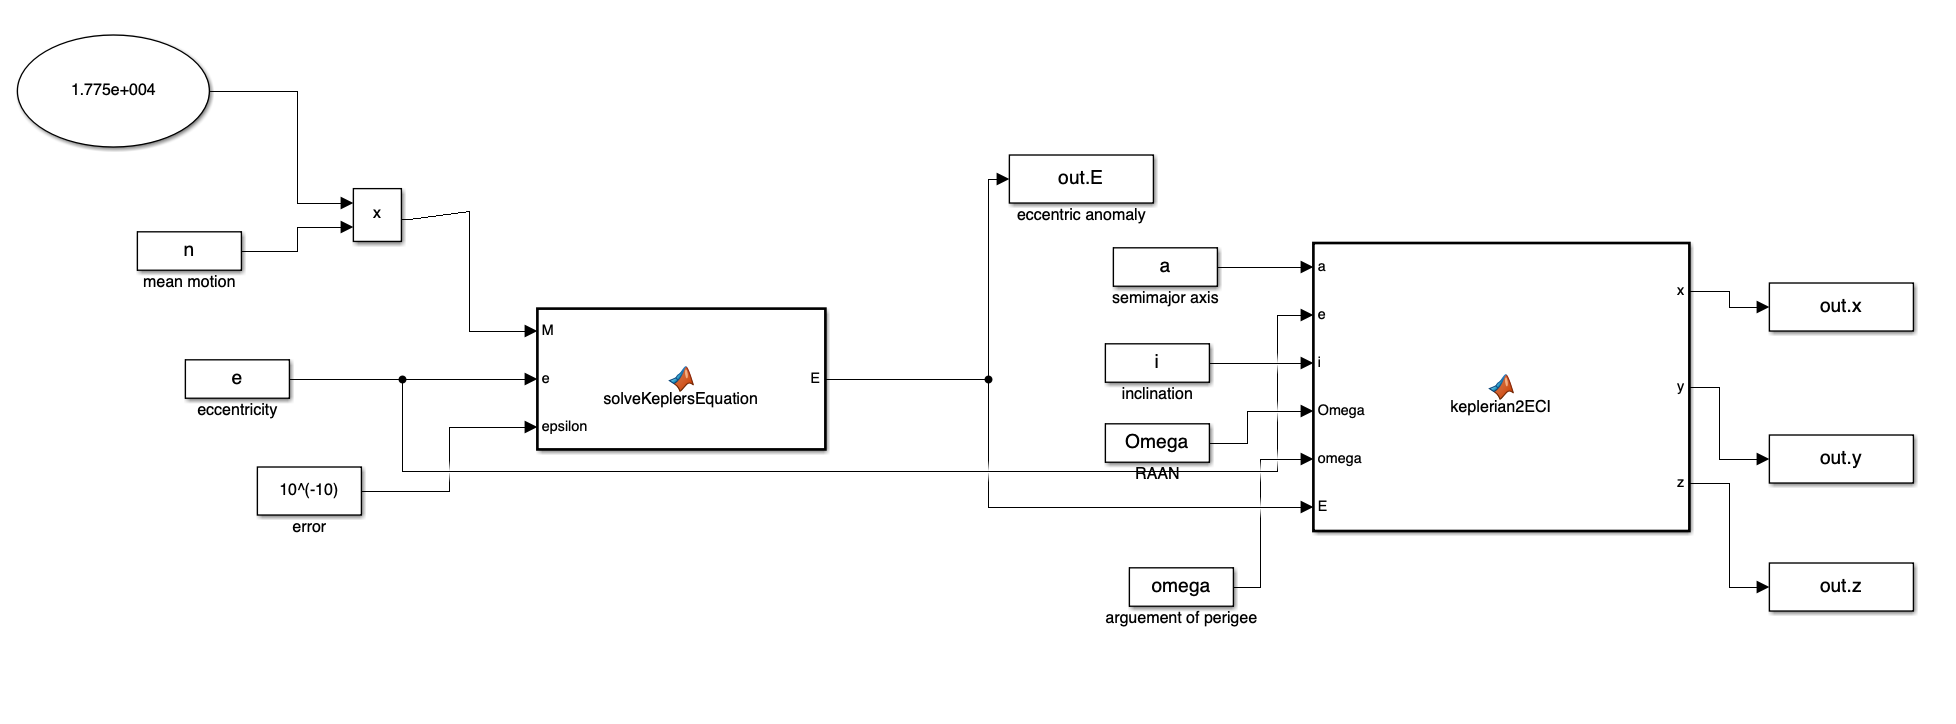
\includegraphics[width = 15.5cm]{Images/simulink_prop.png}
    \caption{Simulink Model for Keplerian Propagator}
    \label{fig:simulink-prop}
\end{figure}

The Keplerian propagator was then used to plot the orbit for a time span roughly equal to three orbital periods. The resulting orbit along with a spherical model of Earth is shown below in Figure \ref{fig:kep_orbit}.

\begin{figure}[H]
    \centering
    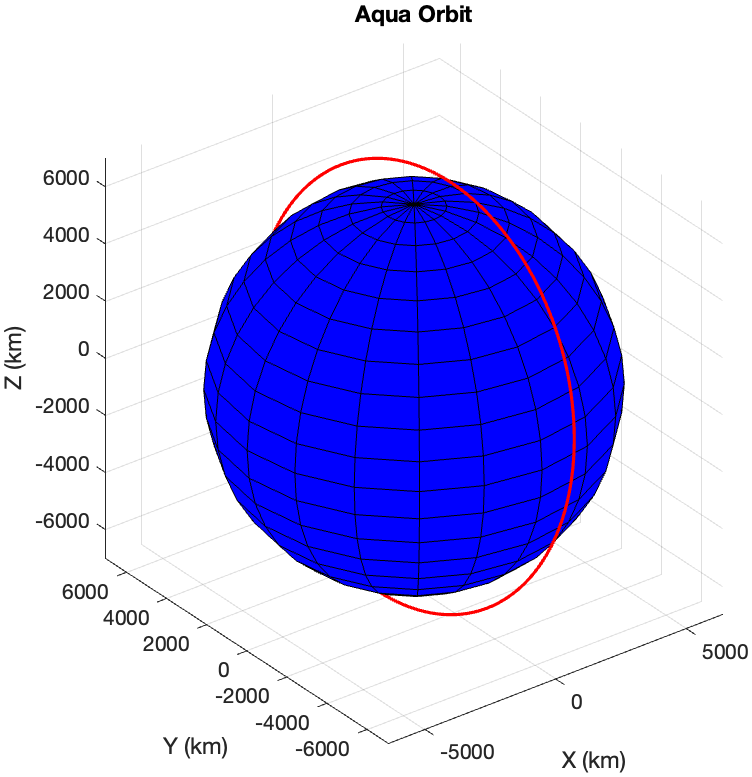
\includegraphics[width = 8.5cm]{Images/aqua_orbit_kepler.png}
    \caption{Aqua Orbit for Keplerian Propagator}
    \label{fig:kep_orbit}
\end{figure}

The Matlab function that was used for the Keplerian propagator can also be seen here.

\lstinputlisting{Code/src/orbit_propogator_kep.m}

Additionally, a numerical propagator was created so that it could be used to account for perturbations and other forces later on in the project. Similarly to the keplerian propagator, the orbital elements were first converted to the initial position and velocity of the spacecraft. From there, the gravitational force of Earth ($\dot v$) and the velocity ($\dot r$) were stacked to created a state vector that could be propagated with a Matlab integrator. The resulting orbit from using a Runge-Kutta method solver is shown below in Figure \ref{fig:numerical_orbit_rk}.


\begin{figure}[H]
    \centering
    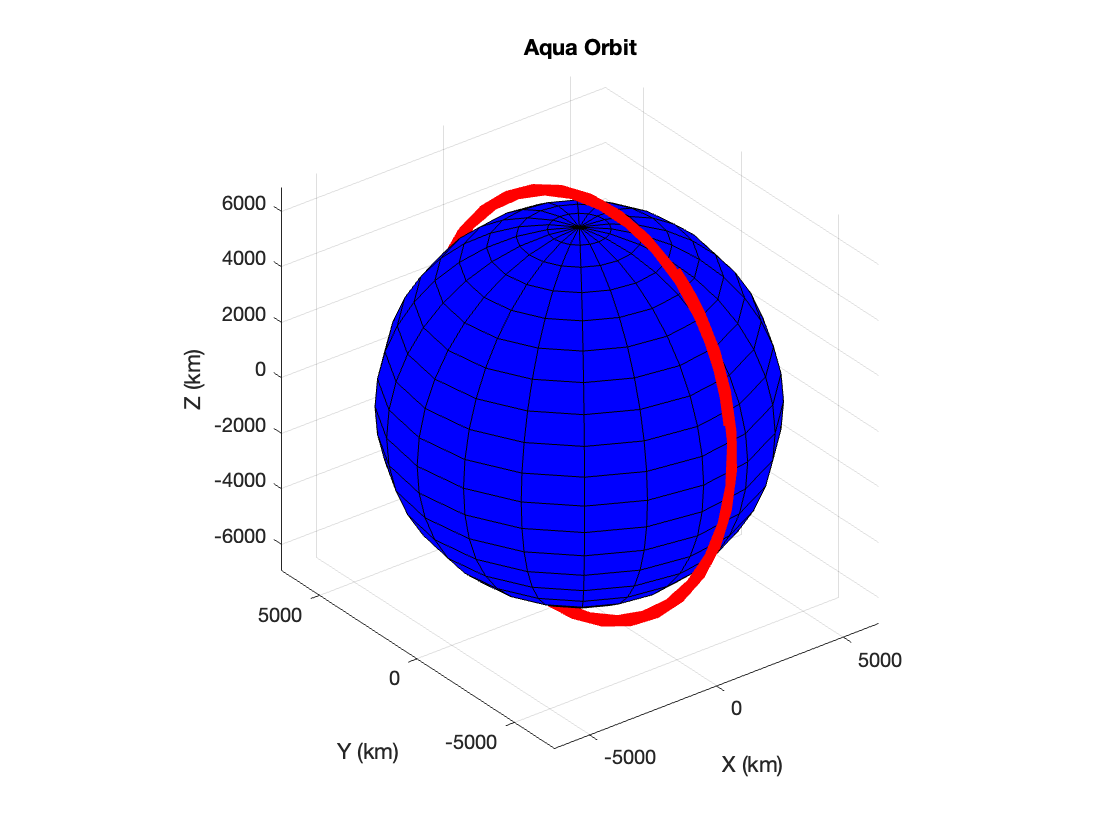
\includegraphics[width = 10cm]{Images/ode45_orbit.png}
    \caption{Aqua Orbit for RK Integrator}
    \label{fig:numerical_orbit_rk}
\end{figure}

Because this integrator resulted in a noticable amount of cumulative error over time, the Adams-Bashforth-Moulton method was also used and is shown below.

\begin{figure}[H]
    \centering
    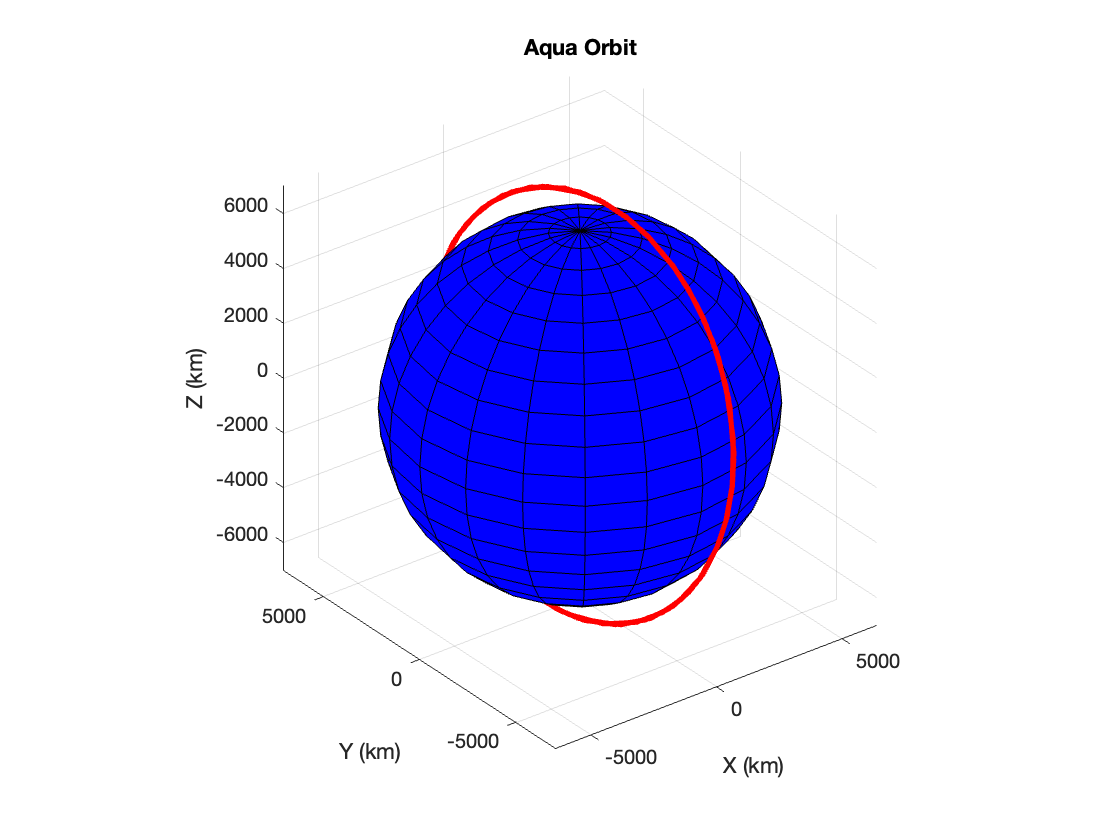
\includegraphics[width = 10cm]{Images/ode23_orbit.png}
    \caption{Aqua Orbit for ABM Integrator}
    \label{fig:numerical_orbit_rk}
\end{figure}

The functions used to obtain these are results are shown below.

\lstinputlisting{Code/src/orbit_propogator_num.m}



\subsubsection{In general the body axes are not the principal axes. Identify principal axes through the eigenvector/eigenvalue problem discussed in class and compute the rotation matrix from body to principal axes.} \label{sec:principal_inertia_def_and_calc}

To resolve an inertia tensor $\boldsymbol{I_{CM}}$ to a diagonal matrix of principal moments of inertia, there must exist a matrix, $\boldsymbol{A}$ such that the Equation \ref{eq:principal_moments} holds, where $\boldsymbol{I_{CM}'}$ is the principal moment of inertia tensor about the center of mass.

\begin{equation} \label{eq:principal_moments}
    \boldsymbol{I_{cm} A} = \boldsymbol{A I_{CM}'} 
\end{equation}

It can be seen that the principal moments of inertia are the eigenvalues of the inertia tensor and that the matrix $\boldsymbol{A}$ is a matrix whose columns are the right eigenvectors of the inertia tensor. For the AQUA spacecraft, the results that follow are shown below.

\begin{equation*}
    \boldsymbol{I_{CM}'} = \begin{bmatrix}
        17510 & 0 & 0 \\
        0 & 23616 & 0 \\
        0 & 0 & 36245
    \end{bmatrix} \text{kg} \cdot \text{m}^2
\end{equation*}

\begin{equation*}
    \boldsymbol{A} = \begin{bmatrix}
            0.0045  &  0.9949 &  -0.1011 \\
            -0.9986  & -0.0007  & -0.0520 \\
            -0.0518  &  0.1012  &  0.9935
    \end{bmatrix}
\end{equation*}

\subsubsection{At this stage you should have a simple 3D model of your spacecraft including geometry and mass properties of each element. This includes at least two coordinate systems, body and principal axes respectively, and the direction cosine matrix between them. Plot axes of triads in 3D superimposed to spacecraft 3D mode}

The body axes of the spacecraft are seen plotted in Figure \ref{fig:aquacad}. The principal inertia axes are seen plotted in Figure \ref{fig:aquacad_principal}.

\begin{figure}[H]
    \centering
    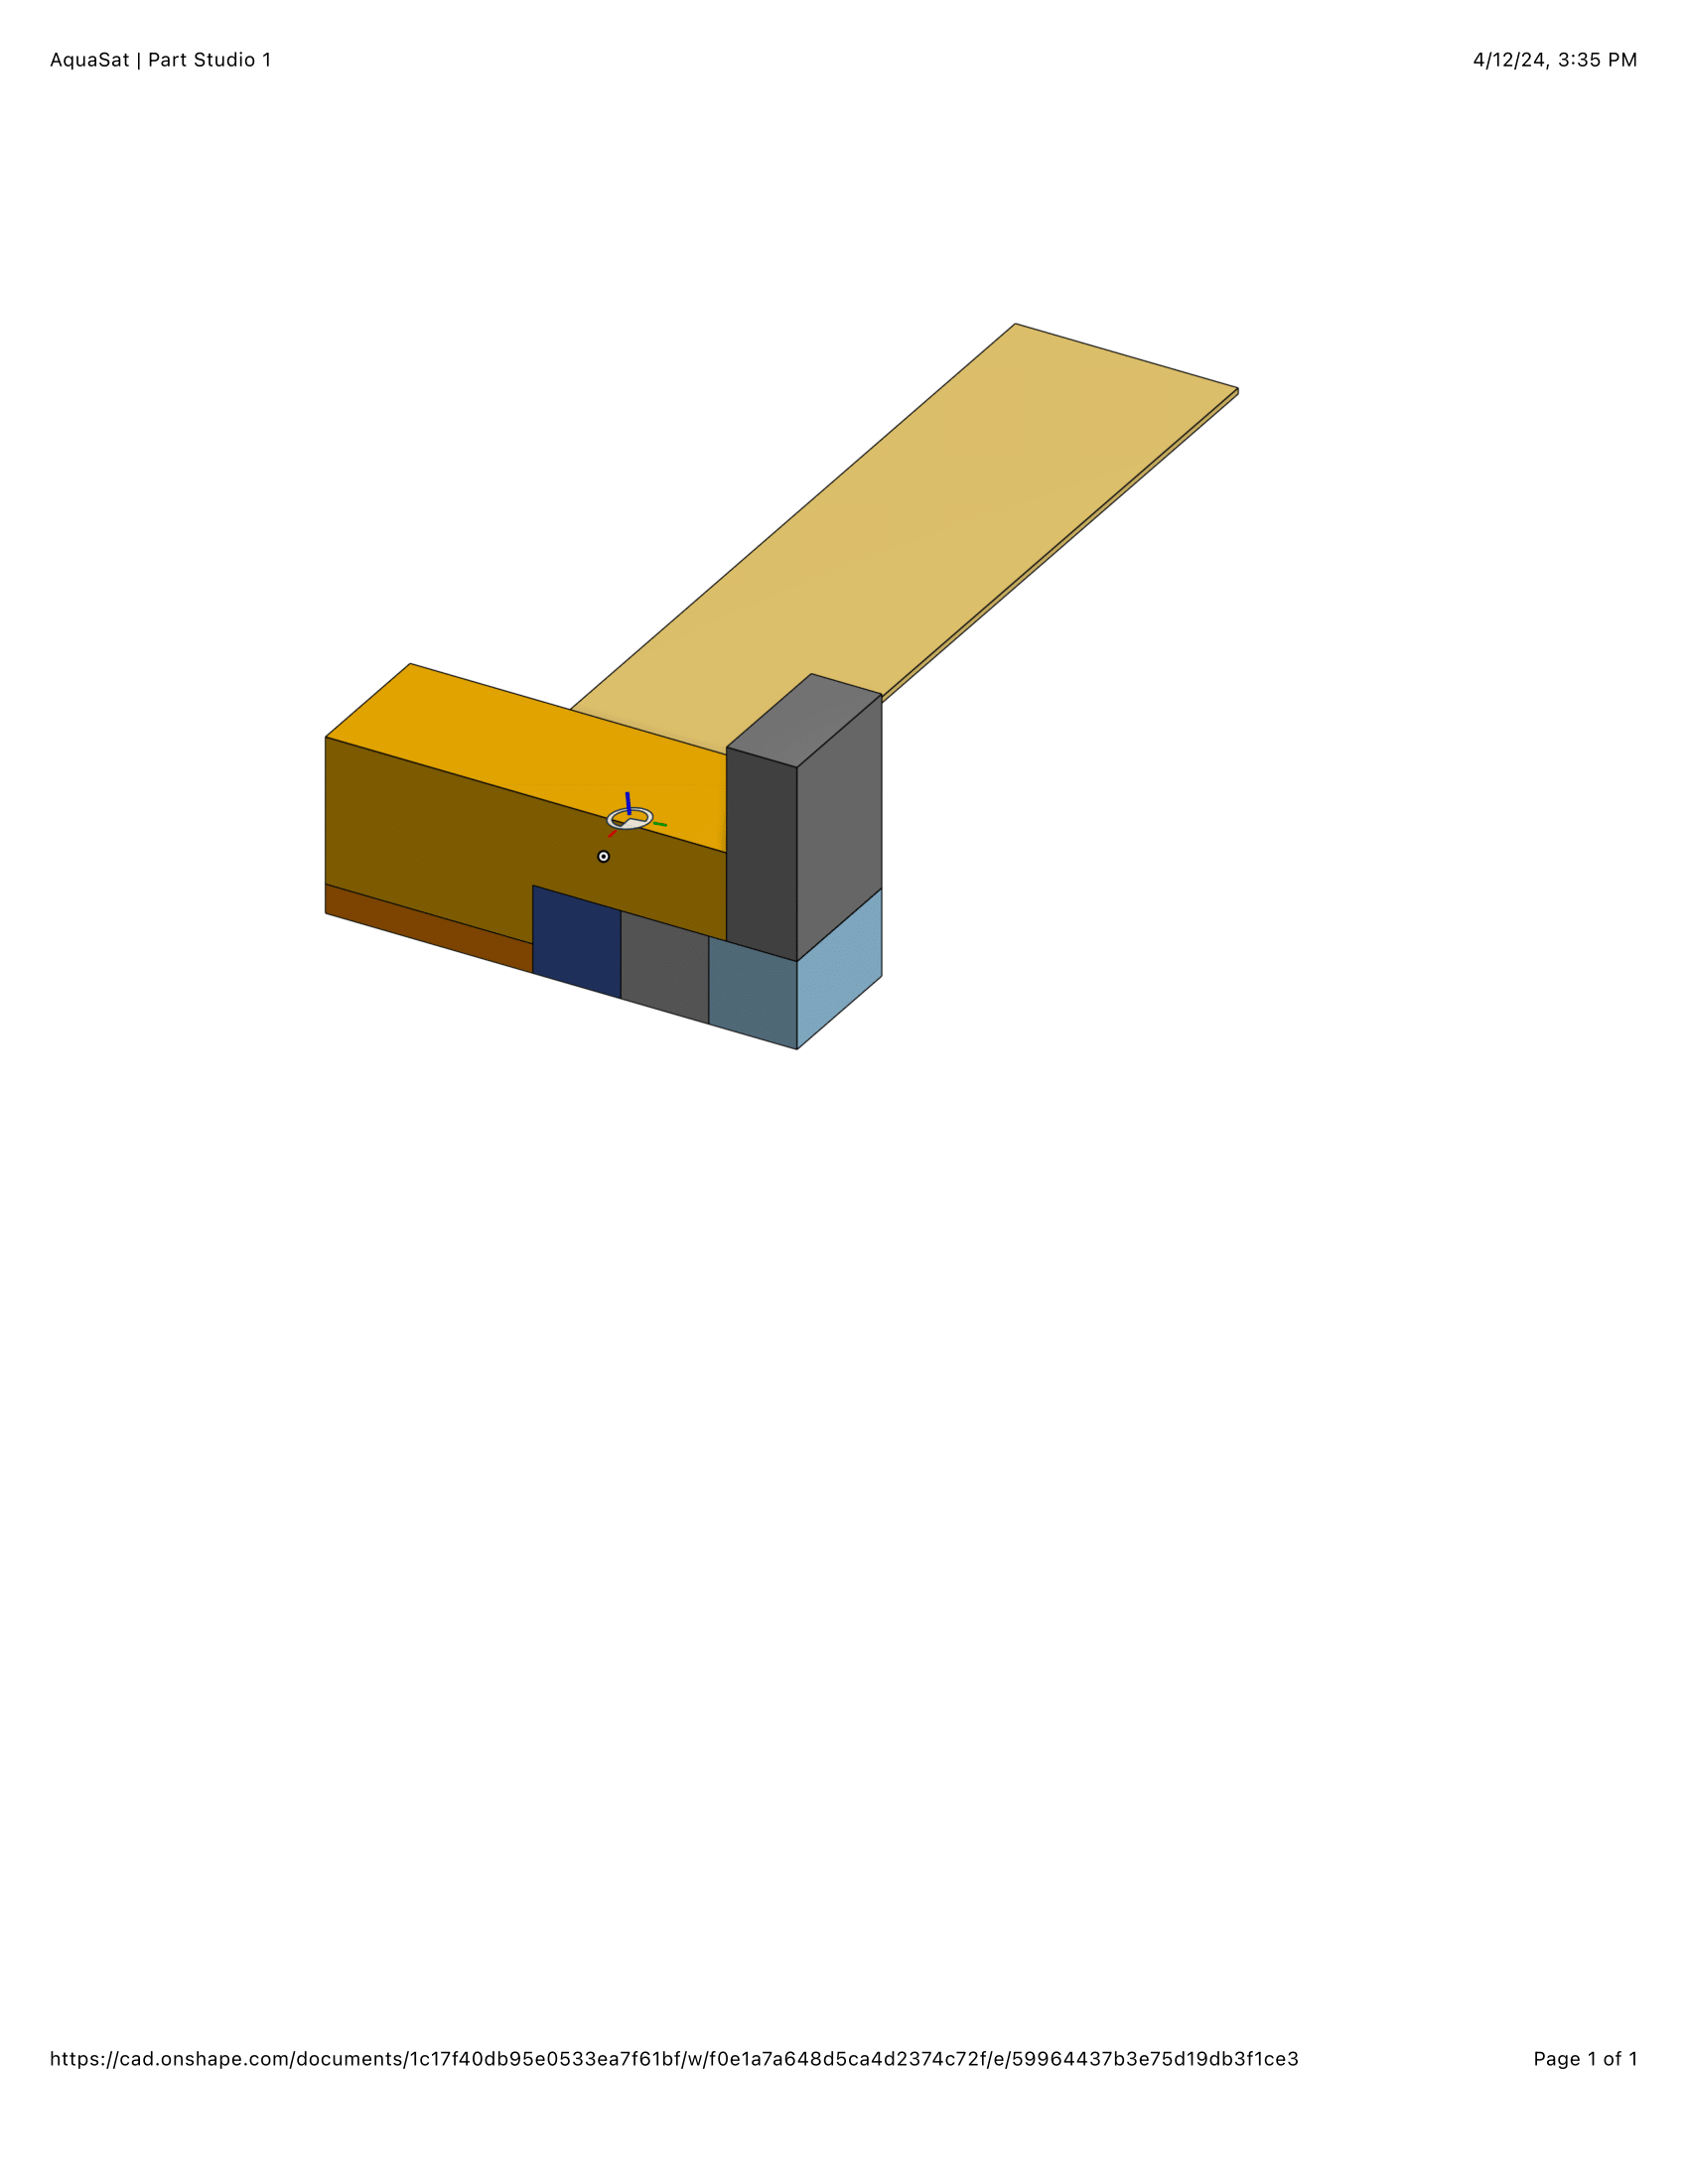
\includegraphics[width = 10cm]{Images/AquaSat_PrincipalAxes.png}
    \caption{Simplified Aqua Model with Principal Axes}
    \label{fig:aquacad_principal}
\end{figure}

\subsubsection{Program Euler equations in principal axes (e.g. in Matlab/Simulink). No external torques.}

The following Simulink model utilizing a MATLAB function (both in Figure \ref{fig:euler_prop_model}) takes in an initial rotational velocity vector and simulates the physics of the current AQUA model about the principal axes of inertia.

\begin{figure}[H]
    \centering
    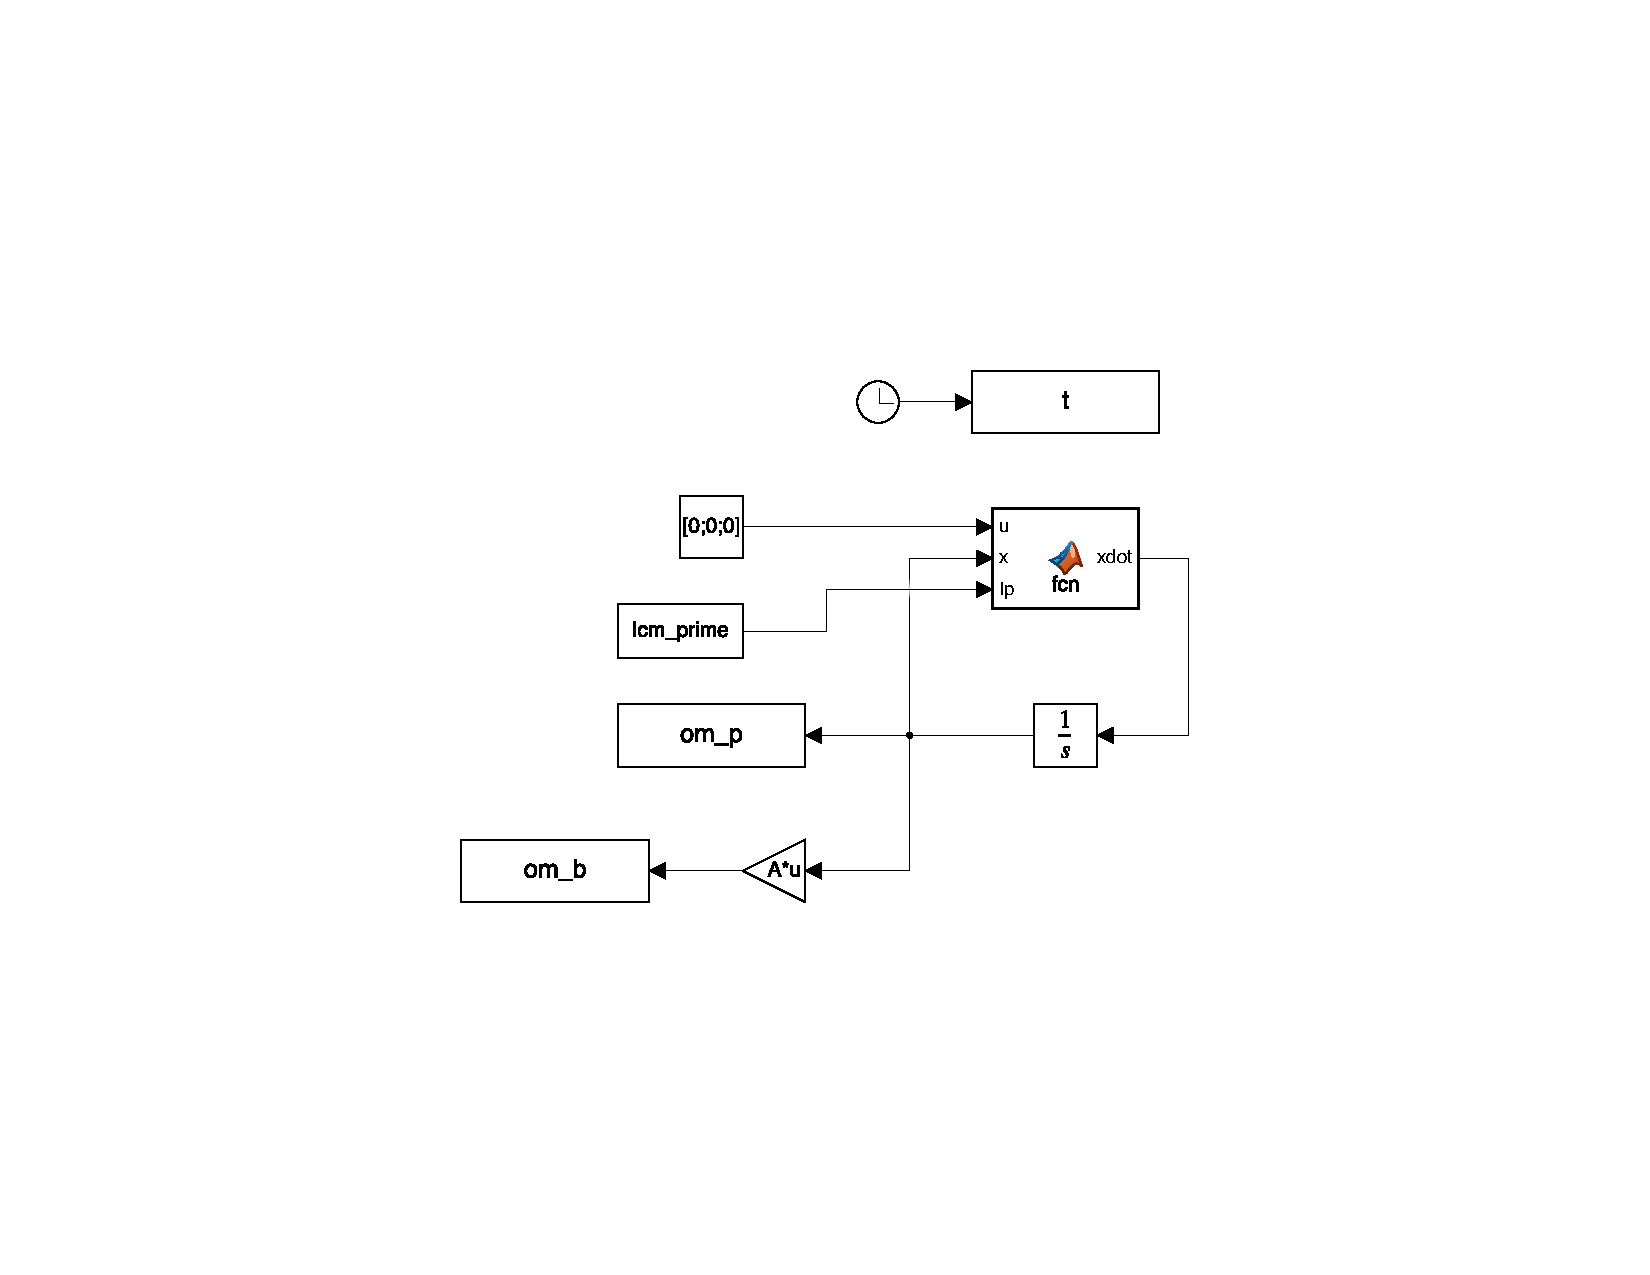
\includegraphics[trim={5cm 5cm 5cm 5cm},clip,width = 15cm]{Images/eulerPropagate.pdf}
\end{figure}

\begin{figure} [H]
    \centering
    \begin{lstlisting}
function xdot = fcn(u,x,Ip)

xdot = zeros(size(x));


Mx = u(1);
My = u(2);
Mz = u(3);

omx = x(1);
omy = x(2);
omz = x(3);

Ix = Ip(1,1);
Iy = Ip(2,2);
Iz = Ip(3,3);

wxdot = (1/Ix)*(Mx - (Iz - Iy)*omy*omz);
wydot = (1/Iy)*(My - (Ix - Iz)*omz*omx);
wzdot = (1/Iz)*(Mz - (Iy - Ix)*omx*omy);

xdot(1) = wxdot;
xdot(2) = wydot;
xdot(3) = wzdot;

end
    \end{lstlisting}
    \caption{Euler Propagation Simulink Model}
    \label{fig:euler_prop_model}
\end{figure}


\subsubsection{Numerically integrate Euler equations from arbitrary initial conditions ($\boldsymbol{\omega < 10^{\circ}/s}$, $\boldsymbol{\omega_i \neq 0}$). Multiple attitude revolutions.}

Given an initial condition of $\vec{\omega}_0 = \begin{bmatrix}
    -7 & 2 & 5
\end{bmatrix}^T {}^{\circ}/s$, gyroscopic coupling causes a periodic oscillation in the angular velocity vector represented in a body fixed axis frame. In this instance in particular, the simulation results shown in \ref{fig:sim_omegas} follows this evolution in the principal frame.

\begin{figure}[H]
    \centering
    \captionsetup{justification = centering}
    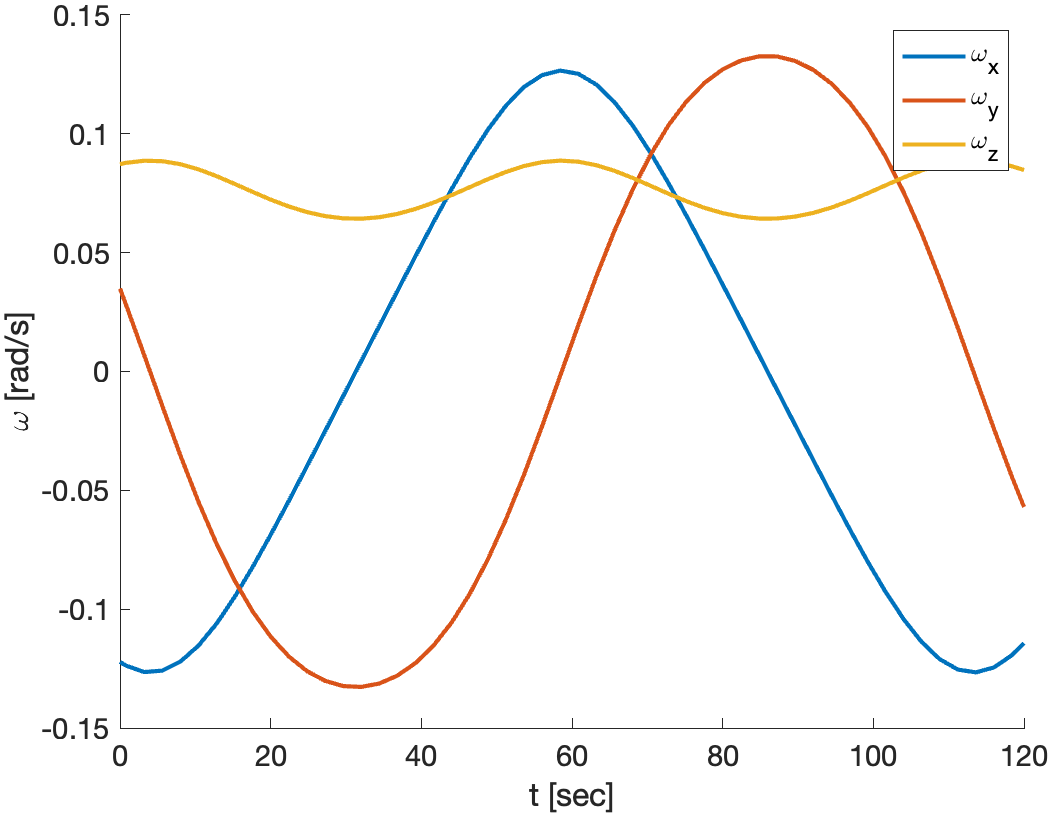
\includegraphics[width = 10cm] {Images/omega_prop_random.png}
    \caption{Angular Velocity Vector Components Evolving in the Body Fixed Principally Oriented Frame}
    \label{fig:sim_omegas}
\end{figure}

\subsubsection{Plot rotational kinetic energy and momentum ellipsoids in 3D (axis equal) corresponding to chosen initial conditions. Verify that semi-axis of ellipsoids corresponds to theoretical values} \label{sec:ellipsoid_definitions}

The angular momentum and rotational kinetic energy of a rigid body is computed using Equations \ref{eq:ang_mom} and \ref{eq:rot_KE} respectively, where $\vec{L}$ and $T$ are the momentum vector and energy, and the angular velocity vector in the principally oriented frame is described as $\vec{\omega} = \begin{bmatrix} \omega_x & \omega_y & \omega_z \end{bmatrix}^T$. 

\begin{equation} \label{eq:ang_mom}
    \vec{L} = \boldsymbol{I_{CM}'}\vec{\omega} = I_x \omega_x + I_y \omega_y + I_z \omega_z
\end{equation}

\begin{equation} \label{eq:rot_KE}
    T = \vec{\omega} \cdot \vec{L} = I_x \omega_x^2 + I_y \omega_y + I_z \omega_z^2
\end{equation}

These quantities are both conserved, so the satellite's angular velocity must always take on a vector value that yields the same momentum magnitude and kinetic energy as the initial conditions. With the initial conditions given above, the magnitude of angular momentum is 3906.4 kg m/s and the kinetic energy is 283.08 J. With not much manipulation, these relations can be shown to be equivalent to Equations \ref{eq:mom_ellipse} and \ref{eq:energy_ellipse} respectively, where L is the magnitude of the angular momentum vector.  

\begin{equation} \label{eq:mom_ellipse}
    \frac{\omega_x^2}{(L/I_x)^2} + \frac{\omega_y^2}{(L/I_y)^2} + \frac{\omega_z^2}{(L/I_z)^2} = 1
\end{equation}

\begin{equation} \label{eq:energy_ellipse}
    \frac{\omega_x^2}{2T/I_x} + \frac{\omega_y^2}{2T/I_y} + \frac{\omega_z^2}{2T/I_z} = 1
\end{equation}

By inspection, the form of these equations is that of an ellipsoid. Therefore, if the Cartesian coordinates are chosen such that the x,y, and z components of the angular velocity lie along the x,y, and z axes, the tip of the angular velocity vector plotted on these axes will lie on the surface of these ellipsoids. The momentum ellipsoid is plotted along with its semi-axis lengths is plotted in Figure \ref{fig:momentum_axis_verification}. The same is done for the energy ellipsoid in Figure \ref{fig:energy_axis_verification}.

\begin{figure}[H]
    \centering
    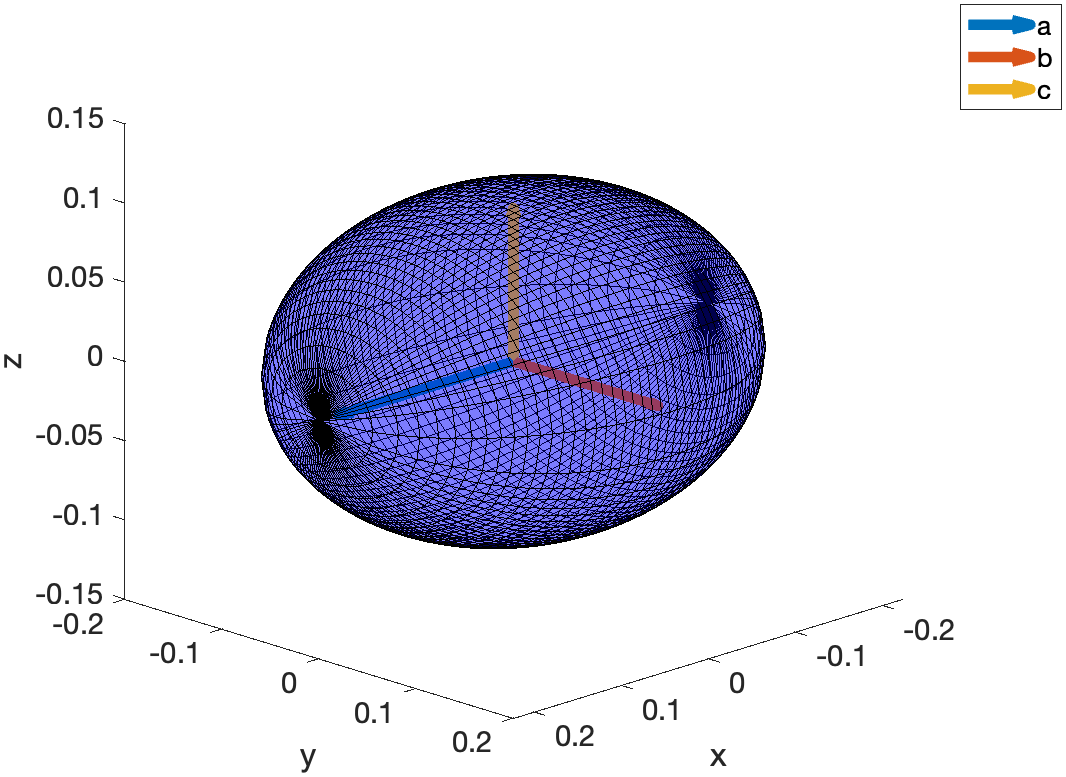
\includegraphics[width = 10cm]{Images/momentum_axes_random.png}
    \caption{Momentum Ellipsoid and Semi-Axis Lengths}
    \label{fig:momentum_axis_verification}
\end{figure}

\begin{figure}[H]
    \centering
    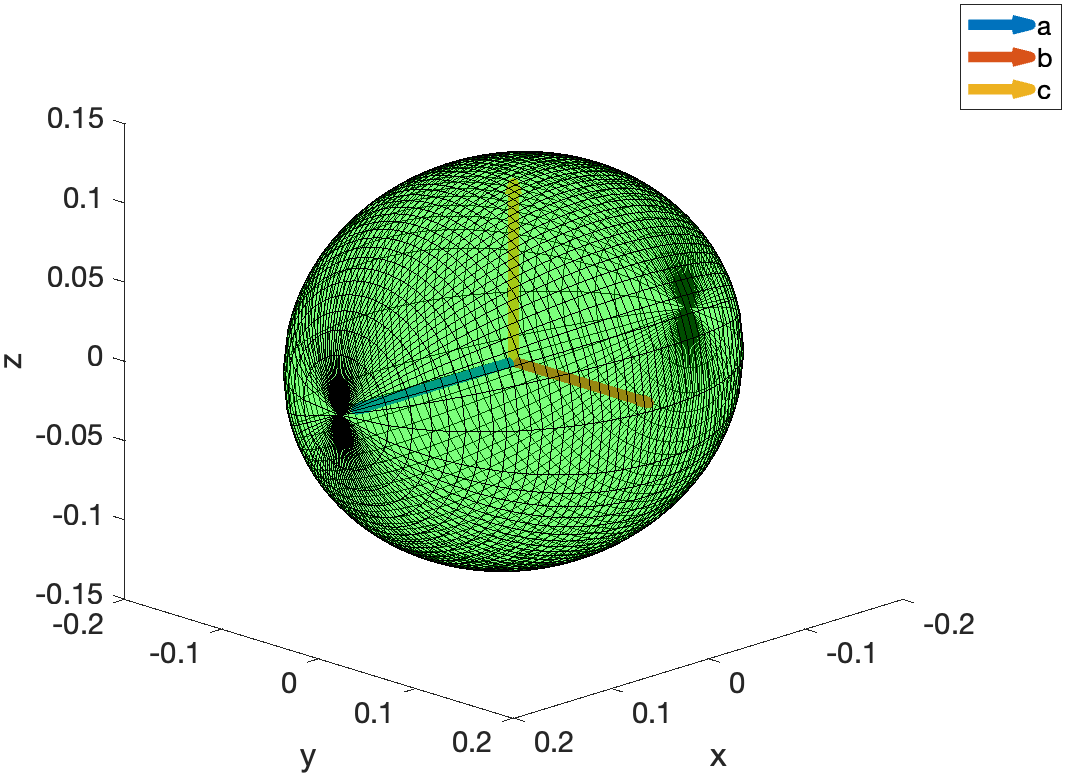
\includegraphics[width = 10cm]{Images/energy_axes_random.png}
    \caption{Energy Ellipsoid and Semi-Axis Lengths}
    \label{fig:energy_axis_verification}
\end{figure}

\subsubsection{Plot polhode in same 3D plot. Verify that it is the intersection between the ellipsoid}

Following that the angular velocity in a Cartesian plot must lie along the surface of both ellipsoids described in Section \ref{sec:ellipsoid_definitions}, it follows that the vector would be restricted to the intersection of the two ellipsoids. The curve that this vector traces is called the polhode, and the simulated results of this curve can be seen in Figure \ref{fig:ellipsoid_super_plot}, over-plotted with the momentum and energy ellipsoids. This curve matches the expected behavior in that it clearly traces the intersection between the momentum and energy ellipsoids. 

\begin{figure}[H]
    \centering
    \captionsetup{justification = centering}
    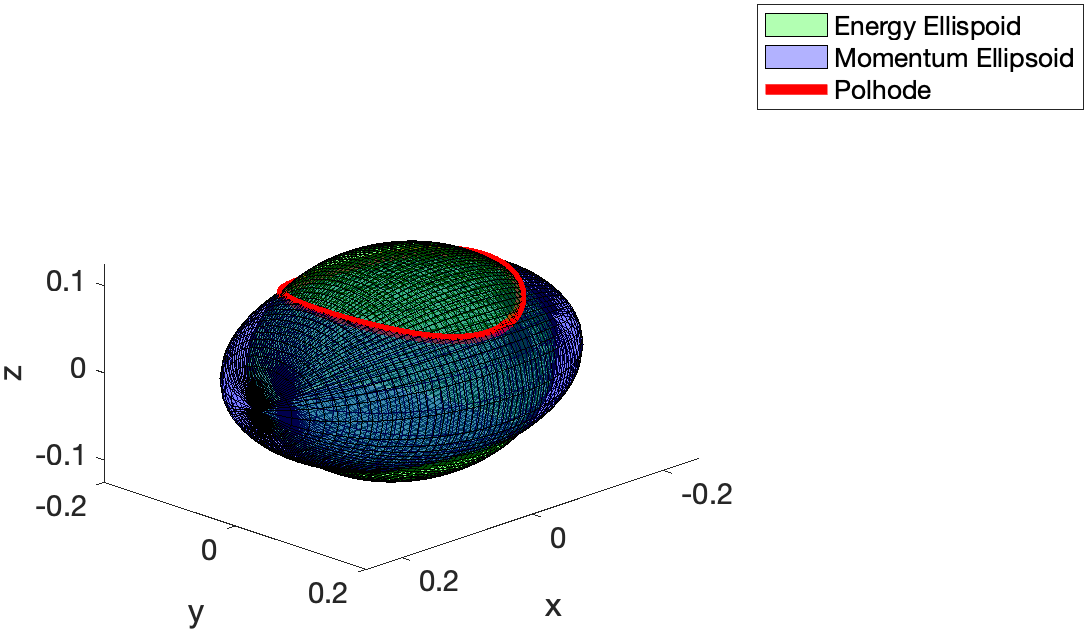
\includegraphics[width = 12cm] {Images/ellipsoid_polhode_random.png}
    \caption{Momentum and Energy Ellipsoids and Polhode Curve Plotted in 3D on Principally Aligned Coordinate Axes}
    \label{fig:ellipsoid_super_plot}
\end{figure}

\subsubsection{Plot polhode in three 2D planes identified by principal axes (axis equal). Verify that shapes of resulting conic sections correspond to theory.}

Figure \ref{fig:2d_polhode} shows the planar projections of the polhode curve along the labeled axes. In theory, these curves should be described by Equations \ref{eq:polhode1}, \ref{eq:polhode2}, and \ref{eq:polhode3}. 

\begin{equation} \label{eq:polhode1}
    (I_y - I_x)I_y \omega_y^2 + (I_z - I_x)I_z \omega_z^2 = L^2 - 2TI_x
\end{equation}

\begin{equation} \label{eq:polhode2}
    (I_x - I_y)I_x \omega_x^2 + (I_z - I_y)I_z \omega_z^2 = L^2 - 2TI_y
\end{equation}

\begin{equation} \label{eq:polhode3}
    (I_x - I_z)I_x \omega_x^2 + (I_y - I_z)I_y \omega_y^2 = L^2 - 2TI_z
\end{equation}

Due to the fact that $I_x < I_y < I_z$, Equation \ref{eq:polhode1} describes an ellipse in the yz plane, Equation \ref{eq:polhode2} a hyperbola in the xz plane, and Equation \ref{eq:polhode3} another ellipse in the xy plane. The theoretical values obtained from these equations were plotted over the polhode that resulted from simulations in Figure \ref{fig:2d_polhode}, establishing that the simulated dynamics followed the expected behavior. Additionally, these equations imply that $I_x < L^2/2T < I_y$. With these initial conditions, this quantity evaluates to 26954 kg m\textsuperscript{2} which lies within the specified bounds described in \ref{sec:principal_inertia_def_and_calc}.

\begin{figure}[H]
    \centering
    \captionsetup{justification = centering}
    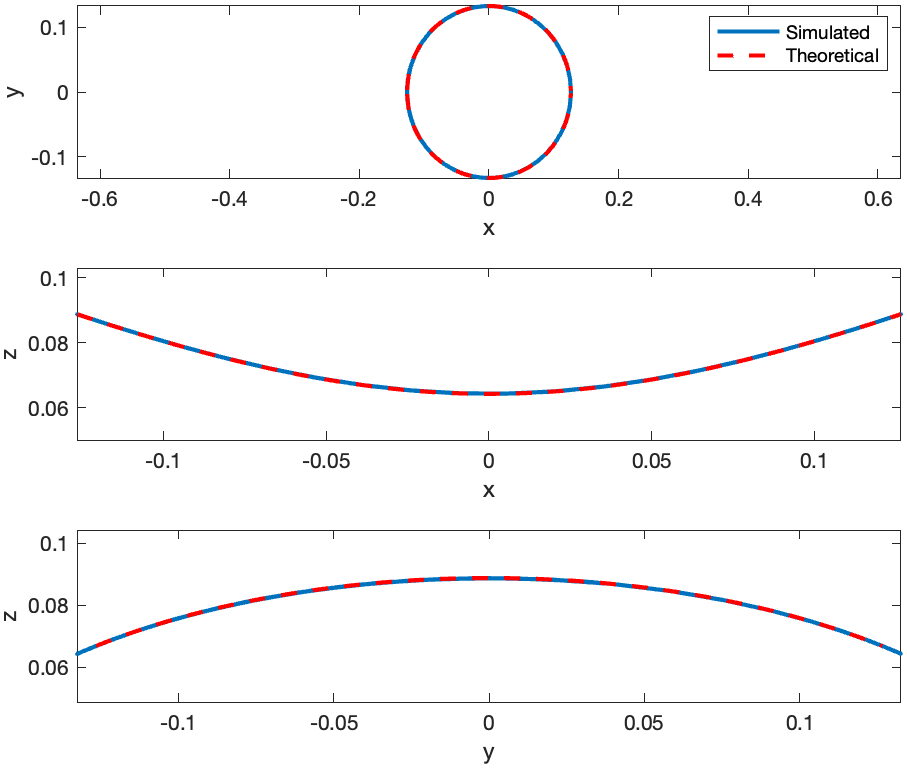
\includegraphics[width = 10cm]{Images/planar_polhode_random.png}
    \caption{Polhode Curve Projected onto Principally Aligned Cartesian Coordinate Planes}
    \label{fig:2d_polhode}
\end{figure}

\subsubsection{Repeat above steps changing initial conditions, e.g. setting angular velocity vector parallel to principal axis. Is the behavior according to expectations?} \label{sec:principally_aligned_omega}

Now with an initial condition of $\vec{\omega}_0 = \begin{bmatrix}
    10 & 0 & 0
\end{bmatrix}^T {}^{\circ}/s$ the magnitude of momentum and kinetic energy are 3056.1 kg m/s and 266.69 J respectively. With the angular velocity vector strictly aligned with one of the principal axes, the vector does not evolve in the principally oriented frame. That is, there is no gyroscopic coupling that causes the zero components of the angular velocity to increase or decrease. The vector components plotted over time are seen in Figure \ref{fig:sim_omegas_principal} 

\begin{figure}[H]
    \centering
    \captionsetup{justification = centering}
    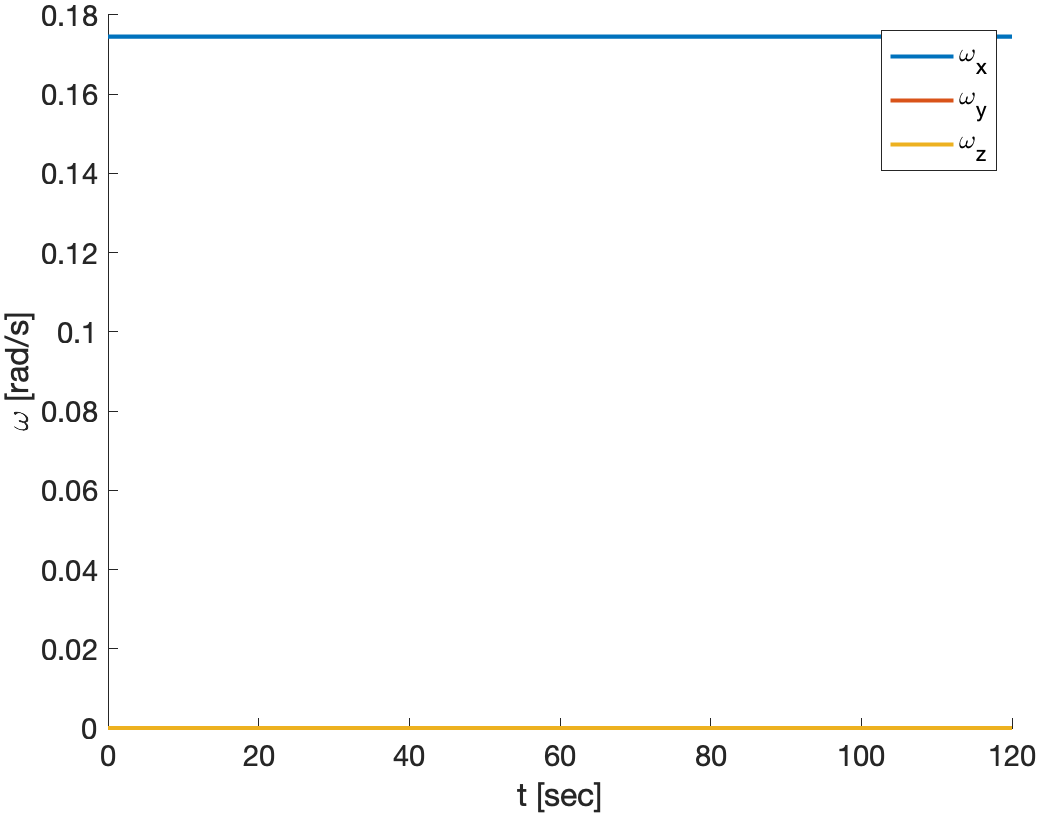
\includegraphics[width = 10cm]{Images/omega_prop_principal.png}
    \caption{Angular Velocity Vector Components for Principally Aligned Initical Conditions}
    \label{fig:sim_omegas_principal}
\end{figure}

The momentum and energy ellipsoids along with their semi-axis lengths can be seen plotted in Figures \ref{fig:momentum_axis_verification_princ} and \ref{fig:energy_axis_verification_princ} respectively.

\begin{figure}[H]
    \centering
    \captionsetup{justification = centering}
    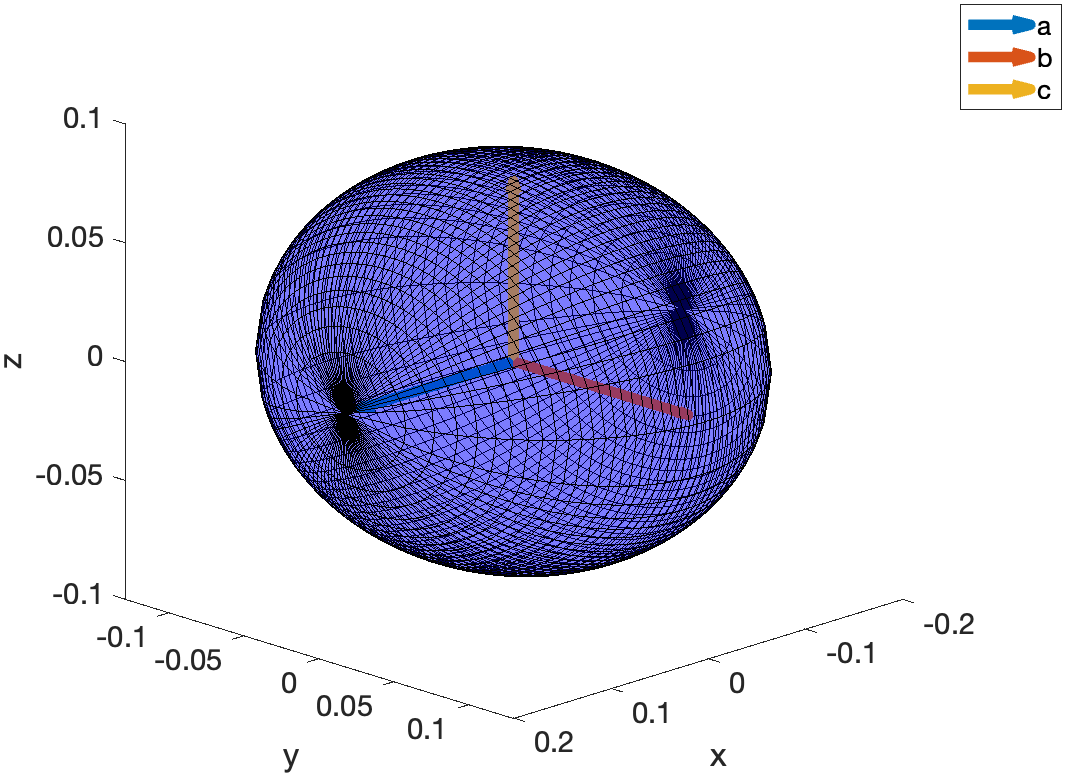
\includegraphics[width = 10cm]{Images/momentum_axes_principal.png}
    \caption{Momentum Ellipsoid and Semi-Axis Lengths for Principally Aligned Velocity Vector}
    \label{fig:momentum_axis_verification_princ}
\end{figure}

\begin{figure}[H]
    \centering
    \captionsetup{justification = centering}
    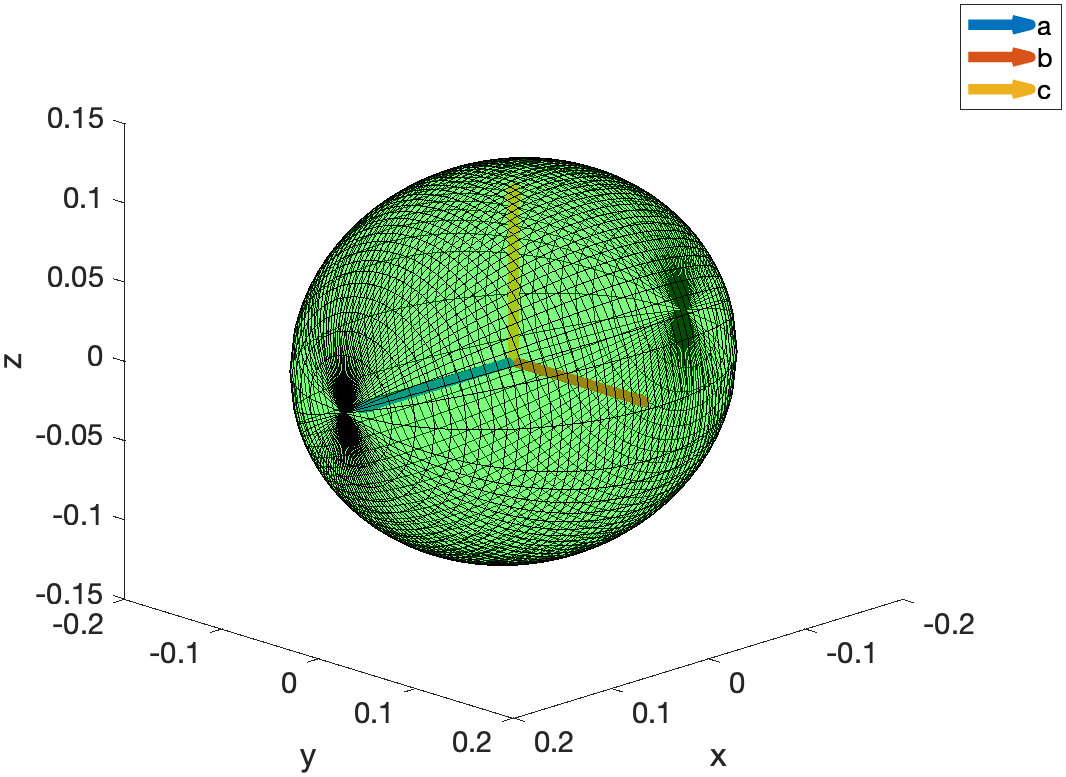
\includegraphics[width = 10cm]{Images/energy_axes_principal.png}
    \caption{Energy Ellipsoid and Semi-Axis Lengths for Principally Aligned Velocity Vector}
    \label{fig:energy_axis_verification_princ}
\end{figure}

This manifests in the polhode graph being a single point. Figure \ref{fig:ellipsoid_super_plot_principal} shows this point plotted at the intersection of the energy and momentum ellipsoids. The intersection in this case is strictly a point as the momentum ellipsoid is fully contained within the energy ellipsoid with two tangent points at  $10^{\circ}/s$ and $-10{}^{\circ}/s$ along the x-axis. 

\begin{figure}[H]
    \centering
    \captionsetup{justification = centering}
    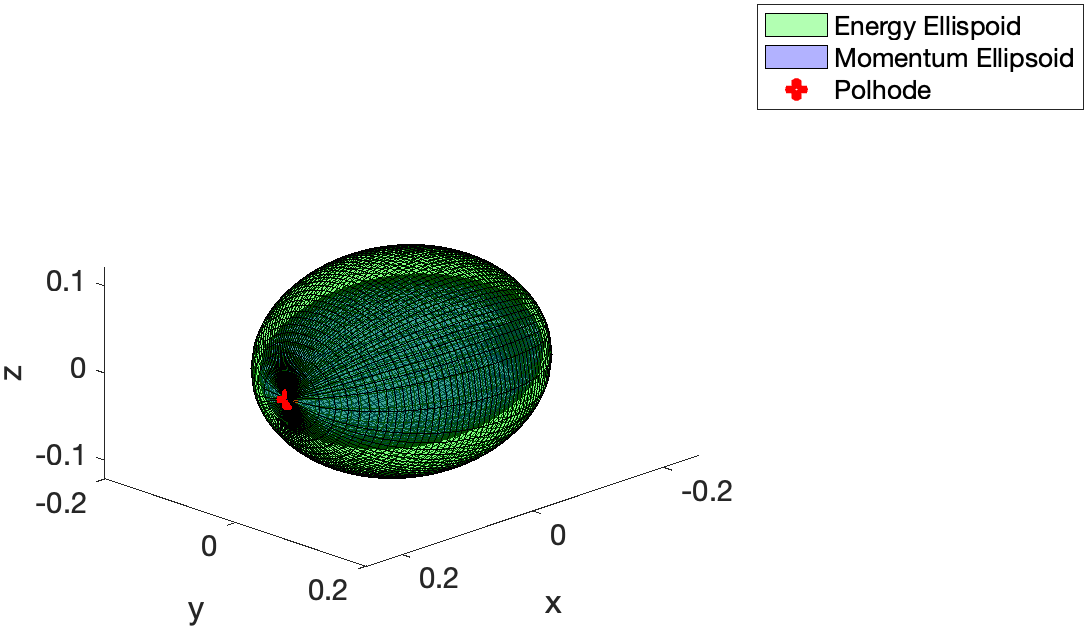
\includegraphics[width = 12cm] {Images/ellipsoid_polhode_principal.png}
    \caption{Momentum and Energy Ellipsoids and Polhode for Angular Velocity Aligned with a Principal Axis}
    \label{fig:ellipsoid_super_plot_principal}
\end{figure}

The polhode projected onto 2D axes is a single point that should lie along the theoretical curve described in Equations \ref{eq:polhode1}, \ref{eq:polhode2}, and \ref{eq:polhode3}. This is shown to hold true in Figure \ref{fig:2d_polhode_principal}. The points from simulation are seen to coincide with the theoretical expectation within an error on the order of magnitude of $10^{-8}$. Additionally, with these initial conditions, the quantity $L^2/2T$ evaluates to 17510 kg m\textsuperscript{2} which lies within the specified bounds described in \ref{sec:principal_inertia_def_and_calc}..

\begin{figure}[H]
    \centering
    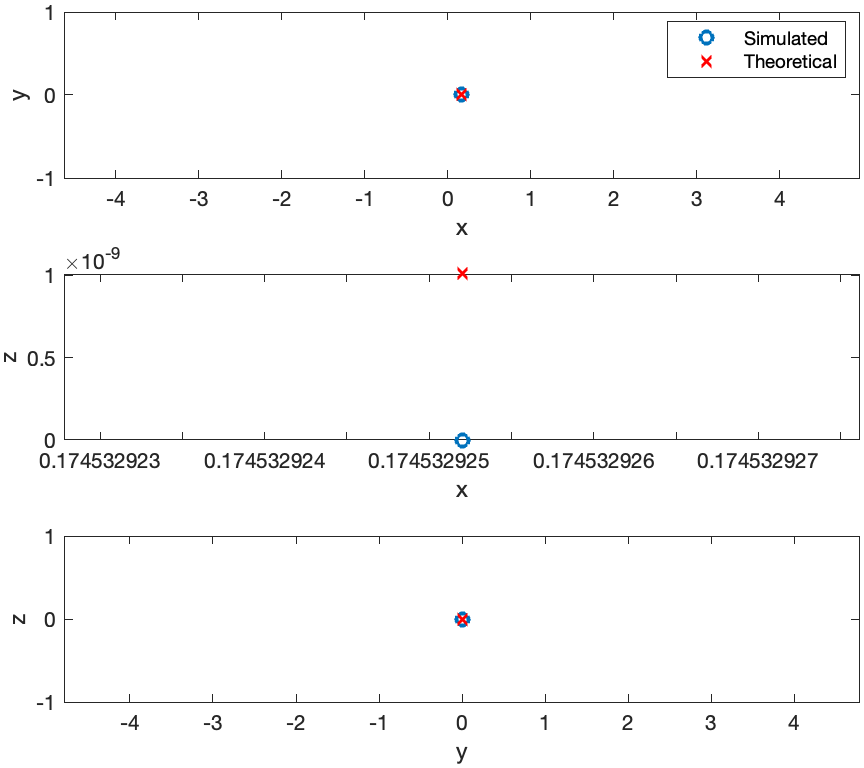
\includegraphics[width = 10cm]{Images/planar_polhode_principal.png}
    \caption{Projected Polhode Curve for Principally Aligned Angular Velocity Vector}
    \label{fig:2d_polhode_principal}
\end{figure}

The code used to perform all calculations and plots for Sections \ref{sec:principal_inertia_def_and_calc} -- \ref{sec:principally_aligned_omega} is listed below.

\lstinputlisting{Code/src/HW2main.m}